\documentclass[12pt]{report}
\usepackage {fancyhdr}
\usepackage{helvet}
\renewcommand{\familydefault}{\sfdefault}
\usepackage{graphicx, amssymb, changepage}
\usepackage{rotating}
\usepackage{setspace}
\usepackage{pgnumchapter_nums}
\usepackage{titlepg}
\usepackage{amsmath}
\usepackage{mathtools}
\usepackage{tocloft} 
\usepackage{url}
\usepackage{booktabs}
\usepackage{hyperref}
\usepackage{indentfirst}
\usepackage{mathrsfs}
\usepackage{algorithm}
\usepackage{algorithmic}
\floatname{algorithm}{algorithm}
\renewcommand{\algorithmicrequire}{\textbf{input:}}
\renewcommand{\algorithmicensure}{\textbf{output:}}
\renewcommand\cftchappresnum{Chapter}
\renewcommand{\cftdot}{}
\cftsetindents{chapter}{0em}{8em} 
\cftsetindents{section}{2em}{6em}
\cftsetindents{subsection}{2em}{6em}
\cftsetindents{subsubsection}{2em}{6em}
\def\listofsymbols{\input{symbols} \clearpage}
\def\addsymbol #1: #2#3{$#1$\> \parbox{5in}{#2 \dotfill  \pageref{#3}}\\}
\def\newnot#1{\label{#1}}
\pagestyle{fancy}
\fancyhead[L,R]{helv \thepage}
\setlength{\headheight}{15.2pt} 
\fancypagestyle{plain}{
	\fancyhf{} % clear all header and footer fields
	\fancyhead{} % clear all header fields
	\fancyfoot{} % clear all footer fields
	\fancyhead[RO]{\thepage}
	\fancyhead[LE]{\thepage}
	\renewcommand{\headrulewidth}{0pt}
	\renewcommand{\footrulewidth}{0pt}
}
\addtolength{\voffset}{-4em}   		
\doublespacing
\lhead{}
\chead{}
\rhead{\thepage}
\lfoot{}
\cfoot{}
\rfoot{}
\renewcommand{\headrulewidth}{0 pt}          %this prints a line under the header
\renewcommand{\footrulewidth}{0  pt}         %this prints a line under the footer
\renewcommand{\contentsname}{\normalsize{Table of Contents}}
\renewcommand{\listfigurename}{\normalsize{List of Figures}}
\renewcommand{\listtablename}{\normalsize{List of Tables}}
\renewcommand{\bibname}{\normalsize{Bibliography}}
\renewcommand{\indexname}{\normalsize{Index}}
\pdfpagewidth 8.5in
\pdfpageheight 11in 
\setlength{\textheight}{8.5in} 
\setlength{\oddsidemargin}{0.5in}  
\setlength{\evensidemargin}{0.5in} 
\setlength{\textwidth}{6.0in}
\setlength{\topmargin}{0.in}    
\setlength{\headheight}{0.5in}
\setlength{\headwidth}{6.0in}
\setlength{\headsep}{0.65in}                   
\setlength{\parindent}{2em}
\graphicspath{{figure/}}
%%%%%%%%%%%%%%%%%%%%%%%%%%%%%%%%%%%%%%%%%%%%
%%%
%%%  This begins the frontmatter of the document, everything preceding the body 
%%%
%%%%%%%%%%%%%%%%%%%%%%%%%%%%%%%%%%%%%%%%%%%%
\begin{document}

\pagenumbering{roman}

\thesistitlepage

\thesiscopyrightpage              
	
\addcontentsline{toc}{chapter}{Abstract}          		 		
\thesisabstract

\addcontentsline{toc}{chapter}{Dedication}  				
\thesisdedicationpage

\addcontentsline{toc}{chapter}{Acknowledgments}   			
\thesisacknowledgments

\makeatletter \renewcommand{\@dotsep}{10000} \makeatother

\renewcommand{\contentsname}{\normalsize{Table of Contents}}    
\tableofcontents

\newpage
\addcontentsline{toc}{chapter}{List of Tables}     			
\listoftables

\newpage
\addcontentsline{toc}{chapter}{List of Figures}
\listoffigures

%%%%%%%%%%%%%%%%%%%%%%%%%%%%%%%%%%%%%%%%%%%%
%%%
%%%  This begins the body of the document
%%%
%%%%%%%%%%%%%%%%%%%%%%%%%%%%%%%%%%%%%%%%%%%%

\newpage
\pagenumbering{arabic}
\chapter{Introduction}
\par Natural living organism intrinsically has an incremental recognition mechanism. As time goes by, new information is passed in via perception organs continuously while existing knowledge keep preserved. Abstracted information, new knowledge, combining with existing knowledge together makes intelligence grow up incessant. Take human being as example, an infant might only be able to recognize parents and food. During his growth, he will learn to recognize more and more objects or people without forgetting his parents. However, most of modern convolutional neural network based artificial systems are unqualified to learning in dynamic settings where all objects classes are unknown at beginning of training or training datasets are evolving regularly with new classes and samples. Popular ways to migrating model to new tasks is to use pre-trained CNNS and adapted them.
\par Fine-tuning\cite{finetune} adjusts the output layer of the original network by replacing it with classes corresponding to the new task or adding new classes to the existing ones. Weights of this new layers are randomly initialized, while all parameters of the network are tuned with the objective for the new task \cite{shmelkov}. Since all parameters are changed over new classes, this framework performance on new task is fantastic however old tasks suffer dramatically. This issue, where a neural network forgets previously learned knowledge when adapted to a new task, is referred to as catastrophic forgetting. It has been known for over a couple of decades in the context of feedforward fully connected networks \cite{chomsky}, and needs to be addressed in the current state-of-the-art object detector networks, if we want to implement incremental learning.
\par Needless to say, as the computer vision systems getting closer towards artificial intelligence, an incremental learning strategy is essential to deal with real-world object vision situation. Using the word incremental, we build a classifier which supports learning new knowledge as well remembering old knowledge.
\begin{figure}
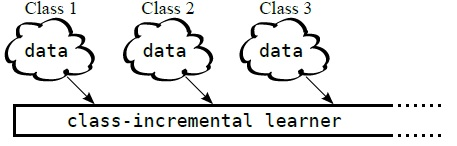
\includegraphics[height = 2in, width = 4in]{1.jpg}
\caption{Class-incremental learning: an classifier learns incessantly new classes as well as old classes from a sequential data stream, who supports multi-class classification on all classes encountered so far.}
\label{fig1}
\end{figure}
\par As shown in Figure\ref{fig1}. It illustrates that at least two properties need to be satisfy as incremental learning:\newline
1. It supports multi-class classification.\newline
2. Training data are feed in from stream so that this model might encounter new class anytime.
\par Although remarkable progress image classification has made recently and some computer vison systems even outperform human experts in specific scenarios like lung cancer detection\cite{cancer}, there is still not a popular satisfying incremental classifier nowadays. Most of existing methods are suffering catastrophic forgetting, a devastating obstacle, leading to prediction accuracy decreasing quickly.
\par In this work, we explore iCaRL(incremental classifier and representation learning)\cite{rebuffi}, a practical strategy for simultaneously learning classifiers and a feature representation in the calss-incremental setting. After repeat iCaRL work, we introduce a new sample algorithm who helps iCaRL get better results. Experiment on CIFAR-10 and CIFAR-100 shows ascensive precision compare with other methods.
\par This paper will review related works in \textbf{Chapter Literature Review}. Details of algorithm are shown in Chapter{Method}. \textbf{Chapter Experiments \& Conclusion} contains discussion of implementation and results. Finally, we make a future plan using iCaRL in \textbf{Chapter Future Work}.
\chapter{Literature Review}
\section{Distilling Knowledge}
\par In 2015, Geoffrey Hinton and his collaborators proposed a mighty method to compress knowledge from existing neural network: Distilling Knowledge\cite{hinton}, providing our incremental algorithm a suitable way to remember exsiting knowledge. Originally, distilling knowledge cames out to reduce computation complexity using a whole ensemble of model. As everyone know, we could always improve the performatnce of any machine learning algorithm by obtaining many different models on same dataset with same target and then averaging their results. This primitive optimization is effective but clumsy. As long as we add more models into our ensemble, computational expenditure grows up linearly. In scientific research, we may still bitter pill to swallow. When deploying real applicaiton, for example autonomous vehicles, which requires model working under limit computation power and deriving results in real time, we can no longer endure large scale model or ensemble models.
\begin{table}
	\centering
	\begin{tabular}{|c|c|c|}
		\toprule
		System & Test Frame Accuracy & WER \\
		\midrule
		Baseline & 58.9\% & 10.9\% \\
		10xEnsemble & 61.1\% & 10.7\%\\
		Distilled Single model & 60.8\% & 10.7\% \\
		\bottomrule
	\end{tabular}
	\caption{Frame classification accuracy and WER showing that the distilled single model performs about as wel as the averaged predictions of 10 models that were used to create the soft targets.}
	\label{tab1}
\end{table}
\par Given such limitations, distilling model could come in handy. Researchers have shown that distilling works very well for transferring knowledge from an ensemble or from a large highly regularized model into a smaller, distilled model. Results for their preliminary experiments on MNIST handwritten digits are shown in Table \ref{tab1}. It proves distillation approach is able to extract more useful information from the training set than simply using the hard labels to train a single label. More than 80\% of the improvement in frame scassification accuracy achieved by using an ensemble of 10 models is transferred to the distilled model which is similar to the improvements we observed in their preliminary experiments on MNIST.
\par To understand intuition behind distilling knowledge needs to understand how distilling works. Typically a classifier usually sets a ``softmax'' layers as last layer which converts a vector $\vec{z}$ into a probability distribution $\vec{q}$ where $q_{i} \in \left(0, 1\right)$, by comparing $z_{i}$ with other digits.
\begin{equation}
	q_{i} = \frac{exp(z_{i} / T)} {\sum_{j}\exp(z_{j}) / T}
\end{equation}
where T is temperature. Using a higher value for T produces smooth distribution over classes. Normally, we consider $q_{i}$ as probability that the object belongs to $class_{i}$. Instead of using original target vector, $\left(\begin{array}{ccccc} 0 \cdots 1 \cdots 000\end{array}\right)$, distilling method uses output, $\left(\begin{array}{cccc}  q_{0} \cdots q_{i} \cdots q_{n - 1}\end{array}\right)$, from softmax layer of large neural network or ensemble of networks as objective. 
\begin{figure}
	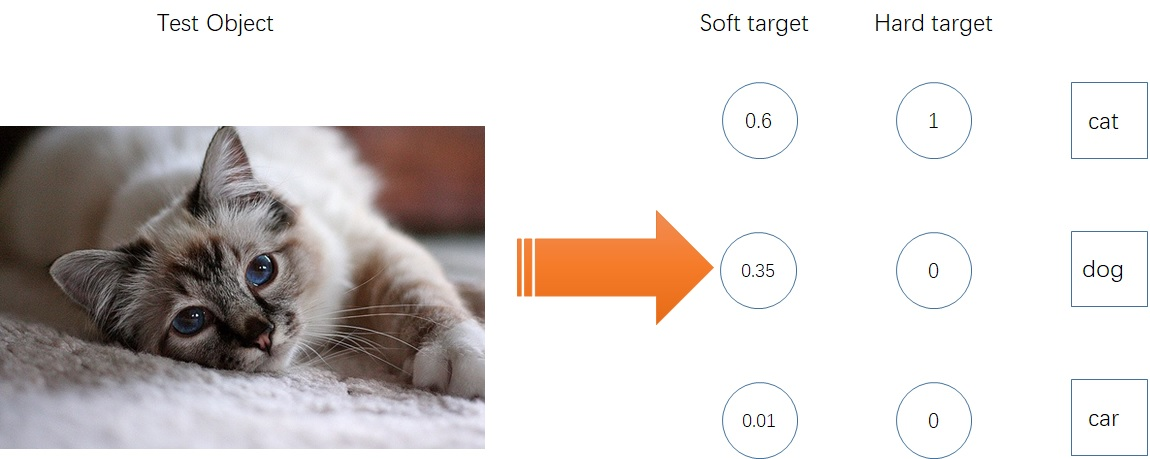
\includegraphics[height = 2.5in, width = 5in]{2.jpg}
	\caption{Soft target, $\left(p_{cat} = 0.6, p_{dog} = 0.35, p _{car} = 0.01\right)$, conveys information that a rich similarity structure over cat and dog, whihe hard target just ignores it.}
	\label{fig2}
\end{figure}
\par Highlight of these ``soft targets'' is that it carries more information than a ``hard target''. We may take a simple classification task as example. Suppose we are classifying targets into three categories: cat, dog and car as shown in Figure\ref{fig2}. Hard target only tells classifier which category dose this image belong to. Meanwhile, soft target conveys not only this image belongs to cat but also define a rich similarity between cat and dog. This is understandable because cat and dog are both animals, more precisely, mammals. Sometimes this kind of feature might not becomprehensible for human being, but it's safe to say, soft target carries much more substantial information than hard original target.
\par Back to topic of incremental learning, it is obviously that we need our system to keep old knowledge in mind. As we discussed above, soft target is good at convey abuntant information. So we naturally implement soft target in our incremental classifier to help system remember old knowledge. Further details about implementation will be elaborated in \textbf{Chapter Literature Review}.
\section{Feature Extracter}
\begin{figure}
	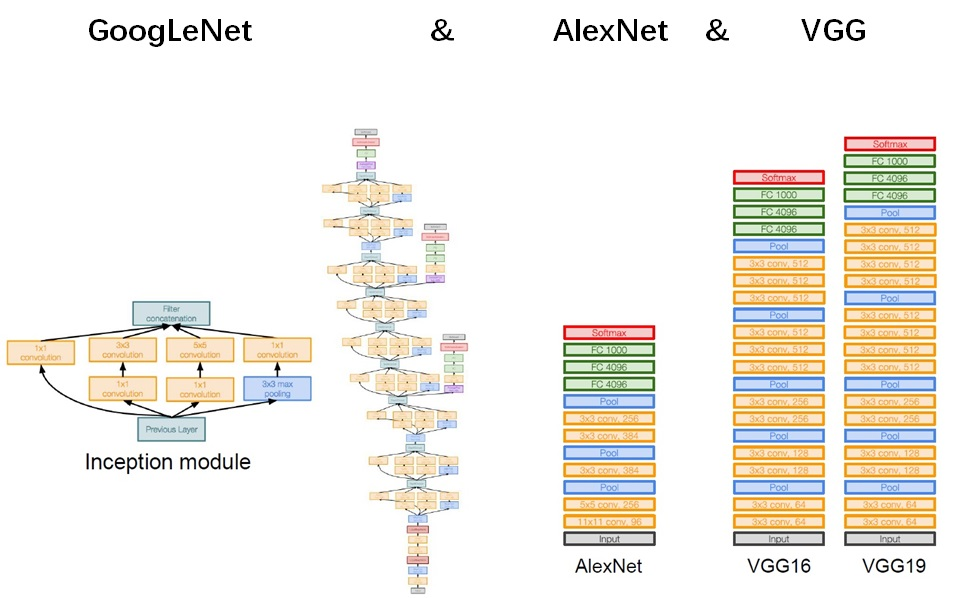
\includegraphics[height = 4in, width = 5in]{5.jpg}
	\caption{Structure of GoogLeNet, AlexNet and VGG}
	\label{fig5}
\end{figure}
\par It no doubt that Convolutional Neural Networks has arouse widely attention in recent years. A bounch of CNN archetectures has shown tremendous power in computer vision problem, and achieved state-of-art results on benchmarks. Imagenet Challenge\cite{imagenet} build a fascinating arena of researchers and their models. Since AlexNet \cite{alexnet} took a gaint leap of deeplearning in 2012, its descendants have break the record of deeplearning again and again including VGG \cite{vgg}, GoogLeNet \cite{googlenet}, ResNet \cite{resnet}, DenseNet \cite{densenet}and so on. In our incremental classifier, we make use of these CNN archetecture as a feature extracter. And all classificaion based on these features.
\begin{figure}
	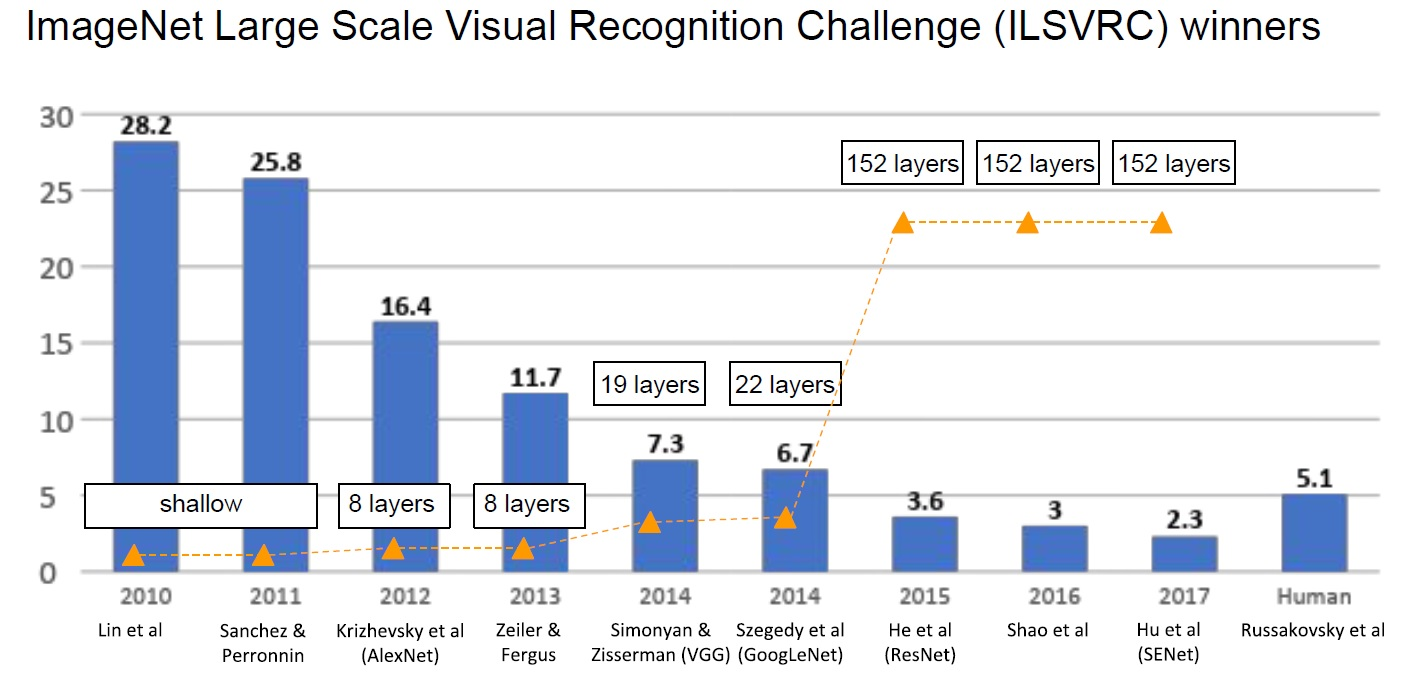
\includegraphics[height = 2.5in, width = 5in]{3.jpg}
	\caption{Comparision of error rate \& depth of different CNN archetecture}
	\label{fig3}
\end{figure}
\begin{figure}
	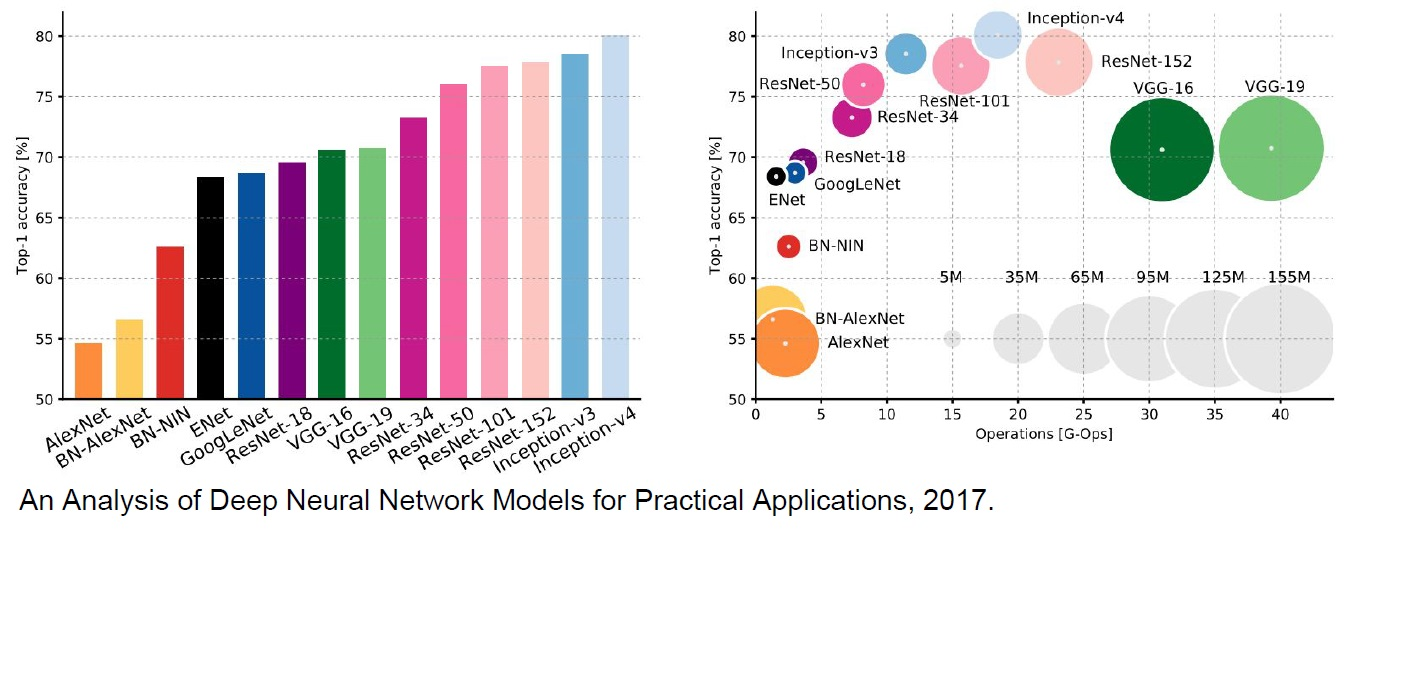
\includegraphics[height = 2.5in, width = 5in]{4.jpg}
	\caption{Comparision of accuracy rate \& number of operation and model size}
	\label{fig4}
\end{figure}
\par First task is to pick up one CNN as our archetecture.Figure\ref{fig3} and Figure\ref{fig4} compares three main properties of these CNN models. Resnet achieves perfect balance between performance and operation time. Due to limit of our computation resource, I choose ResNet as our feature extracter. Figure \ref{fig6} shows basic component of ResNet. Before move on, we should step into details about ResNet.
\begin{figure}
	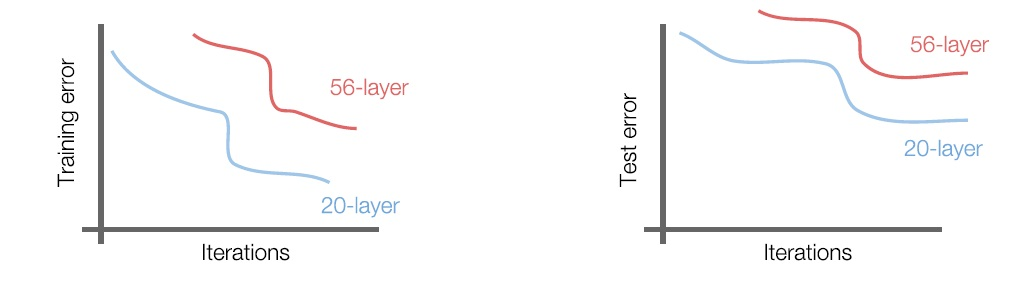
\includegraphics[height = 2in, width = 5in]{7.jpg}
	\caption{56-layer model performs worse than 20-layer model but not because of overfitting!}
	\label{fig7}
\end{figure}
\par As CNN model growing deeper, exploding \cite{exploding} and vanishing \cite{vanishing} gradients always annoy researchers. From Figure \ref{fig7}, we find that sometimes we got worse model if we stack deeper layers on an original convolutional neural network. However, we can imagine that if we manually set those extra convolution layers' kernel weights as 1, at least, deeper model should be able to perform at least as well as the original model. Therefore we are suffering optimization problem due to gradient vanish and explosion. 
\begin{figure}
	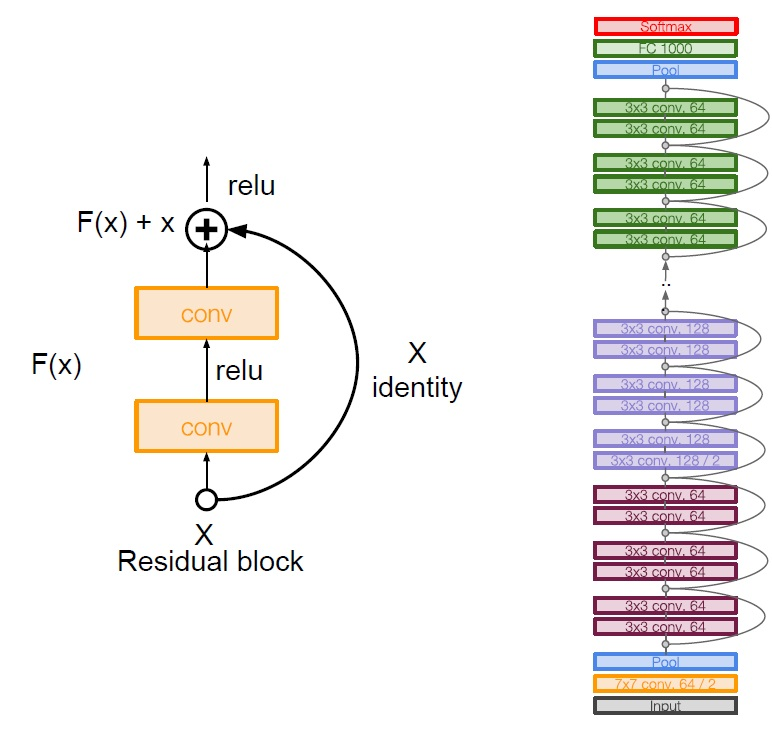
\includegraphics[height = 3in, width = 3in]{6.jpg}
	\caption{Structure of ResNet}
	\label{fig6}
\end{figure}
\par Kaiming He and his collaborators came up a solution that using network layers to fit a residual mapping instead of directly trying to fit desired underlying mapping. In every residual block, original node x not only passes information into common convolution structure but also passes information derectly out current block. Considering relu-layer and convolution layer has highly possible generate large gradient or zero gradient, if we force piece of information flow to next stage, at least we convey some informations rather than lost all of them. This idea can also be found in recent DenseNet. Of course, this structure provides ResNet a solid foundation, achieving a spectacular performance on imagenet. After comprehensive considering, including computational price and performance, we choose ResNet as our feature extracter.

\chapter{Method}

\section{Training Incremental Classifier}
\begin{algorithm}
	\caption{Training}
    \begin{algorithmic}[1]
        \REQUIRE $X = \left( X_{1},\cdots X_{t} \right)$
        \REQUIRE $\Theta$
        \REQUIRE $P = \left(P_{1},\cdots P_{s-1} \right)$
        \STATE $\Theta \leftarrow$ UpdateFeatureExtracter($X,P,\Theta$)
        \FOR{$y = s, \cdots, t$}
        \STATE $P_{y} \leftarrow$ ExamplarConstruction
        \ENDFOR
        \ENSURE $P$
	\end{algorithmic}
\end{algorithm}
\par During training, our system receive new classes of images dynamically from data stream. In every training step, we will combine new data with existing examplar set, recording old knowledge. This makes sure every training step will fully consider existing knowledge. To put it simply, we could just combine new data with examplar set and treat examplar set and new data equally. But as we discussed in previous chapter, we already know a soft target bahave much better than hard target, so it's not strange we trying to make use of soft target. This requires us to carefully design a loss function to describe model error.
\par Under the hood, our system use ResNet18 as our feature extracter. We interpret the network as a trainable extractor, $\varphi \left( x \right): x \rightarrow R^{d}$, followed by a fully connected layer with sigmoid function. And all feature vectors are $L^{2}$ normalized. In all of pseudocode, we use $\Theta$ representing parameters of this network. Finally, outputs from RenNet and fully connected layer are,
\begin{equation}
	\begin{split}
		& \vec{g_{y}} = 1 / \left( 1 + e^{-a_{y} \left( x \right)}\right) \\
		& a_{y} \left( x \right) = w^{T} \varphi \left( x \right)
	\end{split}
\end{equation}
where $w$ stands for weights in fully connected layer. Note that although many classifier uses outputs from sigmoid making prediction, we just use these output to compute loss function and train network.
\par As we have promised, our loss function makes use of soft target.
\begin{equation}
    \begin{split}
        \mathcal{L} =& \mathcal{L}_{classification} + \mathcal{L}_{distillation} \\
        \mathcal{L}_{classification} =& \sum_{y = s}^{t} \delta_{y = y_{i}} \log \left( g_{y}\left(x_{i}\right) \right) + \delta_{y \ne y_{i}} \log \left( 1 - g_{y}\left(x_{i}\right) \right) \\
        \mathcal{L}_{distillation} =& \sum_{y = s}^{t} q_{i}^{y} \log \left( g_{y}\left(x_{i}\right) \right) + \left( 1 - q_{i}^{y}\right) \log \left( 1 - g_{y}\left(x_{i} \right) \right)
    \end{split}
\end{equation}
In fact, this loss function is still a cross entropy \cite{entropy} loss since we could view $\delta$ function as hard target. The only difference is for those data from examplar set, refer to as known classes, we use soft target computed by previous feature extractor. I believe this little change leads us to a totally different training strategy other than fine tuning. The first term, classification loss, leads the network fitting itself to classification task on new classes. At the same time, distillation loss, ensures that the discriminative information of previous classes is not lost suddendly. Once we settle up problem of loss function. Remain training task is totally same as other Convolution Neural Network. We may choose a fimiliar optimizer from Adam \cite{adam}, RMSprop \cite{rms} or SGD \cite{sgd}.
\par In conclusion, we take two measures to avoid catastrophic forgetting. First, we build examplar set to save original information. Second, we make use of distilling knowledge to help system get abundant indent information.  
\begin{algorithm}
	\caption{UpdateFeatureExtracter}
    \begin{algorithmic}[1]
        \REQUIRE $X = \left( X_{1},\cdots X_{t} \right)$
        \REQUIRE $\Theta$
        \REQUIRE $P = \left(P_{1},\cdots P_{s-1} \right)$
        \STATE $D \leftarrow \{ x,y: x \in X \} \bigcup \{ x,y : x \in P \} $
        \FOR{$y = 1, \cdots, s-1$}
        \STATE $\vec{q_{n}} \leftarrow g \left(x_{n} \right): x_{n} \in D$ 
        \ENDFOR
        \STATE $\mathcal{L} \leftarrow \mathcal{L} \left( \{x \in X\}\right)$
        \STATE BackProp
        \STATE Update $\Theta$
	\end{algorithmic}
\end{algorithm}

\section{Nearest Mean Classification}
\begin{algorithm}
	\caption{Classify}
	\begin{algorithmic}[1]
        \REQUIRE $x$
        \REQUIRE $P = \left(P_{1},\cdots P_{t} \right)$
        \REQUIRE $\varphi: x \rightarrow R^{d}$
        \FOR{$y = 1, \cdots, t$}
        \STATE $u_{y} \leftarrow \varphi \left( p \right)$ where $p \in P_{y}$
        \ENDFOR
        \STATE $y^{*} \leftarrow argmin ||\varphi \left( x \right) - u_{y}||$
        \ENSURE class label $y^{*}$
	\end{algorithmic}
\end{algorithm}
\par Our system uses a nearest mean of exemplars classification strategy. Everyone time a test image passed in, feature extracter computes mean feature vector for each classes we met so far: $u_{y} \leftarrow \varphi \left( p \right)$ where $p \in P_{y}$. Then test image will labelled as the class whose mean feature is most similar in $L^{2}$ space. Nearest mean classifier itself is a classic method that can be count as grandfather of recent CNN based method. But it circumnavigate an important barrier in incremental scenario naturally. Ordinary classifier are usually ends with one fully connected layer followed by a sigmoid activation function. No matter what kind of archetecture are used, we still could recognize it as a non-linear projector combining with a linear classifier. In such archetecture, once feature extactor, non-linear projector, has been changed, fully connected layer must be changed as well. Otherwise, we might get a random result. On the contrary, nearest exemplar mean classifier does not rely on fully connected layer, which means the change on feature space is somehow simultaneously. The robustness brought by nearest exemplar helps our system a lot to fight againest feature space changing. Taking advantage from nearest mean method is inspired by Mensink's work on distance-based image classification \cite{near}.

\section{Examplar Construction}
\begin{algorithm}
	\caption{ExamplarConstruction}
    \begin{algorithmic}[1]
        \REQUIRE $X = \{ x_{i} \in y\}$
        \REQUIRE $\varphi: x \rightarrow R^{d}$
        \STATE $u \leftarrow \bar{\varphi \left( x\right)}$
        \STATE $P^{'} \bigcup argmin ||\varphi_{x} - u||: x \in X$
        \STATE $P \leftarrow P \bigcup P^{'}$
        \ENSURE $P_{y}$
	\end{algorithmic}
\end{algorithm}
\par Alogorithm 4 describe the protoset construction construction process. For each new class we met, we first compute the overall mean of all images' features who belongs to this new class. Suppose we want to construct a exemplar set with size k. Then we just pick the first k images who's distance between mean is small. We have to say, this is quiet a rough method. In fact, this is a problem of choose smaples from datset to best describing or representing original large dataset. Other potential methods for exemplar maybe useful. Though we are now use the most simple rule to choose samples, we will keep working on this further problem and better result is expecting.

\chapter{Experiments \& Conclusion}

\chapter{Future Work}

\chapter{Summary}
\par In this work, I explore iCaRl, a strategy for class incremental learning that learns classifier and feature representation simultaneously. 
\newpage
\bibliographystyle{IEEEbib}
\addcontentsline{toc}{chapter}{Bibliography}
\bibliography{pengyu_ref}
\end{document}
 
